\documentclass{beamer}

% !TEX root = ./main.tex
% The above line is a magic comment that tells text editors which file to compile.

\documentclass{beamer}
\usepackage[utf8]{inputenc}
\usepackage{hyperref}
\usepackage{amsmath}
\usepackage{cleveref}
\usepackage{adjustbox}
\usepackage{mathtools}
\usepackage{dsfont}
\usepackage{xcolor}
\usepackage{amsthm}

\usepackage{tikz}
% \usetikzlibrary{arrows.meta}
% \usetikzlibrary{shapes}
% \usetikzlibrary{calc}
% \usetikzlibrary{math}
% \usetikzlibrary{decorations.pathreplacing,calligraphy}
% \usepackage{pgffor}

% \usepackage{algorithm}
% \usepackage{algpseudocode}

\usepackage{macros}
\usepackage{domainmacros}
%%%%%%%%%%
% Beamer %
%%%%%%%%%%

\definecolor{cPurple}{RGB}{124, 0, 133}
\definecolor{cBlue}{RGB}{56, 0, 138}
\definecolor{cRed}{RGB}{180, 0, 60}
\definecolor{cGreen}{RGB}{0, 156, 27}

\usetheme[sectionpage = none, subsectionpage = simple]{metropolis}
\usecolortheme{seahorse}

\usebeamercolor{normal text}
\usebeamercolor{background canvas}

\setbeamercolor{alerted text}{fg=cPurple}

\setbeamertemplate{footline}{%
      \raisebox{8pt}{\makebox[\paperwidth]{\scriptsize \hfill \insertframenumber/\inserttotalframenumber \hspace{5pt}}}}

% \setbeamertemplate{footline}{\raisebox{8pt}{\hfill \insertframenumber/\inserttotalframenumber \hspace{5pt}}}

% \setbeamertemplate{footline}{%
%       \raisebox{8pt}{\makebox[\paperwidth]{\scriptsize \hspace{5pt}  TCS101 \hfill \insertframenumber/\inserttotalframenumber \hfill CC-BY-SA \hspace{5pt}}}}

\beamertemplatenavigationsymbolsempty

\title[RBSR]{Range-Based Set Reconciliation}
\author{Aljoscha Meyer}
\date{}

\begin{document}

\frame{\titlepage}

\begin{frame}{Set Reconciliation}
    \begin{itemize}
        \item set union over a network
        \item between (exactly) two machines
        \item unstructured data
        \item no shared state or history
    \end{itemize}
\end{frame}

\begin{frame}{Trivial Reconciliation}
    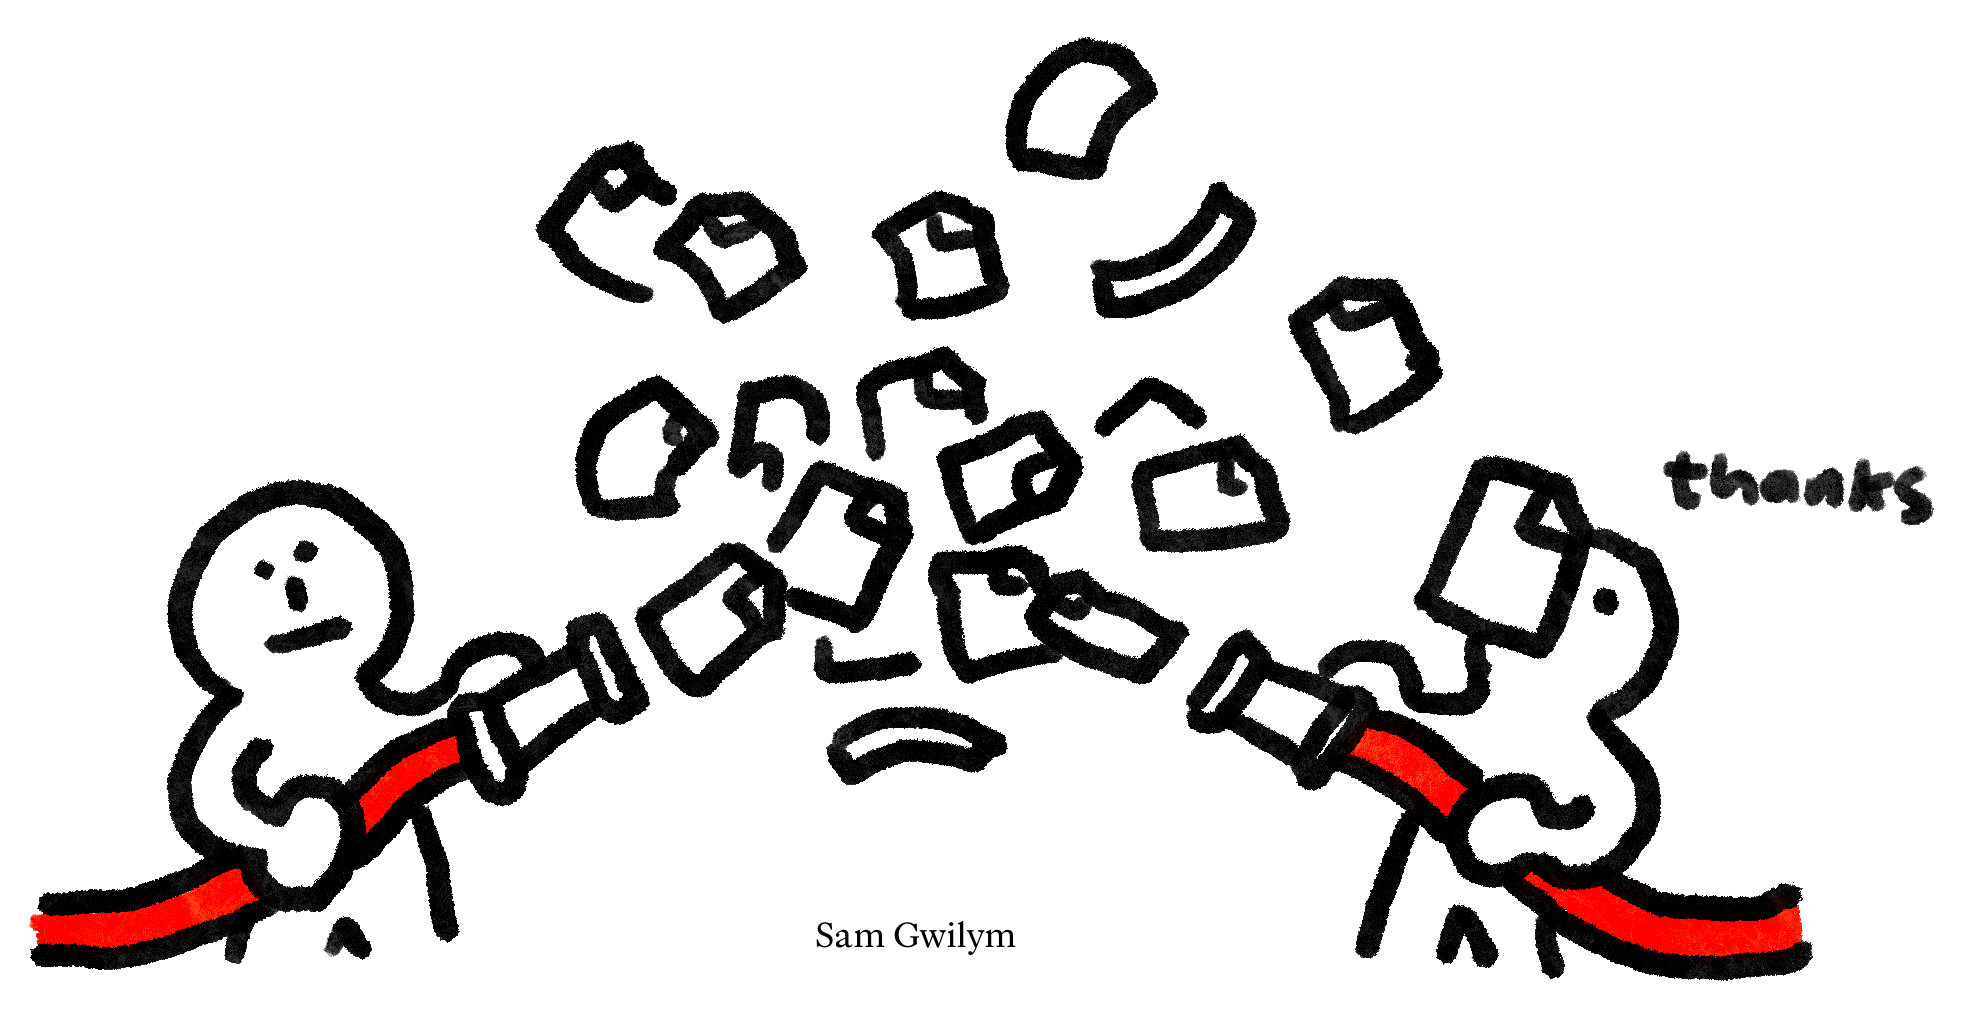
\includegraphics[keepaspectratio=true,width=11.4cm]{trivial_sync.png}
\end{frame}

\begin{frame}{Model and Analysis}
    \begin{itemize}
        \item Alfie and Betty talk over a network
        \item reliable communication, rounds of unit length, unlimited bandwidth
        \item probabilistic solutions \pause
        \item $n$: size of the union
        \item $n_{\triangle}$: size of the symmetric difference
    \end{itemize}
\end{frame}

\begin{frame}{Model and Analysis}
    \begin{itemize}
        \item roundtrips
        \item communicated bytes
        \item computation time
        \item computation space
    \end{itemize}
\end{frame}

\begin{frame}{Traditional Approaches}
    \begin{itemize}
        \item obtain approximation of $n_{\triangle}$
        \item compute message of size $\complexity{n_{\triangle}}$ by iterating over all $n$ items
        \item exchange messenges
        \item recover symmetric difference from those messages using at least $\complexity{n_{\triangle}}$ time and memory
    \end{itemize}
\end{frame}

\begin{frame}{P2P Reconciliation}
    Peer-to-peer systems:
    \begin{itemize}
        \item iterating over local set every time infeasible
        \item loading local set into memory infeasible
        \item some peers are out to get us
    \end{itemize}

    \pause

    $\implies$ traditional approaches don't work
\end{frame}

\begin{frame}{Reducing Computational Complexities}
    \begin{itemize}
        \item allow for logarithmic number of rounds\pause
        \item compare fingerprints of local sets\pause \begin{itemize}
            \item if equal, we are done
        \end{itemize}\pause
        \item divide-and-conquer\pause \begin{itemize}
            \item chose predicate for partitioning\pause
            \item restrict to simple predicates (split into ranges)\pause
            \item peers alternatingly choose splits that are optimal for themselves
        \end{itemize}\pause
        \item binary-search for differences\pause \begin{itemize}
            \item collaboratively
            \item over the wire
            \item in parallel
            \item ok, the analogy is not perfect
        \end{itemize}
    \end{itemize}
\end{frame}

\begin{frame}{Range-Based Set Reconciliation}
    $X_{\alpha} \defeq \{\exampleb, \examplec, \exampled, \examplee, \examplef, \exampleh \}$    
    \hfill
    $X_{\beta} \defeq \{\examplea, \examplee, \examplef, \exampleg\}$
    \begin{tikzpicture}[xscale=0.68, font=\footnotesize]
        \pgfdeclarelayer{background}
        \pgfdeclarelayer{foreground}
        \pgfsetlayers{background,main,foreground}
    
        \begin{pgfonlayer}{main}
            %vertices
            \node (vroot) at (0, 1) [fpi] {\examplefpi{\examplea}{\examplei}{\{\examplea, \examplee, \examplef, \exampleg\}}};

            \only<2->{
                \node (v00) at (-4, -0) [fpi] {\examplefpi{\examplea}{\examplee}{\{\exampleb, \examplec, \exampled\}}};
                \node (v01) at (4, -0) [fpi] {\examplefpi{\examplee}{\examplei}{\{\examplee, \examplef, \exampleh\}}};
            }    
    
            \only<3->{
                \node (v10) at (-4, -1) [iis] {\exampleiis{\examplea}{\examplee}{\{\examplea\}}{0}};
            }
            \only<4->{
                \node (v11) at (2, -1) [fpi] {\examplefpi{\examplee}{\exampleg}{\{\examplee, \examplef\}}};
                \node (v12) at (6, -1) [iis] {\exampleiis{\exampleg}{\examplei}{\{\exampleg\}}{0}};
            }
    
            \only<5->{
                \node (v20) at (-4, -2) [iis] {\exampleiis{\examplea}{\examplee}{\{\exampleb, \examplec, \exampled\}}{1}};
            }
            \only<6->{
                \node (v21) at (6, -2) [iis] {\exampleiis{\exampleg}{\examplei}{\{\exampleh\}}{1}};
            }
            %edges
            \only<2->{
                \draw (vroot) edge[edge] (v00);
                \draw (vroot) edge[edge] (v01);
            }
    
            \only<3->{
                \draw (v00) edge[edge] (v10);
            }
            \only<4->{
                \draw (v01) edge[edge] (v11);
                \draw (v01) edge[edge] (v12);
            }
    
            \only<5->{
                \draw (v10) edge[edge] (v20);
            }
            \only<6->{
                \draw (v12) edge[edge] (v21);
            }
        \end{pgfonlayer}
    
        \begin{pgfonlayer}{background}
            \draw[-{Triangle[width=30pt,length=17pt,color=gray]}, line width=15pt, color=gray](8, 1) -- (-8, 1);
            \only<2->{
                \draw[-{Triangle[width=30pt,length=17pt,color=gray]}, line width=15pt, color=gray](-8, -0) -- (8, -0);
            }
            \only<3->{
                \draw[-{Triangle[width=30pt,length=17pt,color=gray]}, line width=15pt, color=gray](8, -1) -- (-8, -1);
            }
            \only<5->{
                \draw[-{Triangle[width=30pt,length=17pt,color=gray]}, line width=15pt, color=gray](-8, -2) -- (8, -2);
            }
        \end{pgfonlayer}
    \end{tikzpicture}
\end{frame}

\begin{frame}{Some Nice Properties}
    \begin{itemize}
        \item reasonably efficient: $\complexity{\min(n_{\triangle} \cdot \log(n), n)}$ bytes communication, $\complexity{1}$ working memory
        \item can tune bandwidth vs roundtrip minimization
        \item arbitrary recursion anchor protocols
        \item arbitrary partition techniques \pause
        \item but: linear computation times
    \end{itemize}
\end{frame}

\begin{frame}{Reducing Computation Times}
    \begin{itemize}
        \item $\binom{n}{2}$ possible subranges $\implies$ cannot precompute all fingerprints\pause
        \item free space budget of $\complexity{n}$
        \item labeled trees!
    \end{itemize}
\end{frame}

\begin{frame}{Intermission --- Merkle Search Trees}
    Auvolat, Alex, and François Taïani. "Merkle search trees: Efficient state-based CRDTs in open networks." 2019 38th Symposium on Reliable Distributed Systems (SRDS). IEEE, 2019.

    \begin{itemize}
        \item define a unique tree shape for every set
        \item use that shape for a Merkle tree of your set
        \item only exchange fingerprints for ranges that correspond to subtrees
    \end{itemize}
    \pause
    Problems:
    \begin{itemize}
        \item easily attacked with degenerate tree shapes
        \item peers cannot optimize data representation for their use-case
    \end{itemize}
\end{frame}

\begin{frame}{Say No to Merkle Trees}
    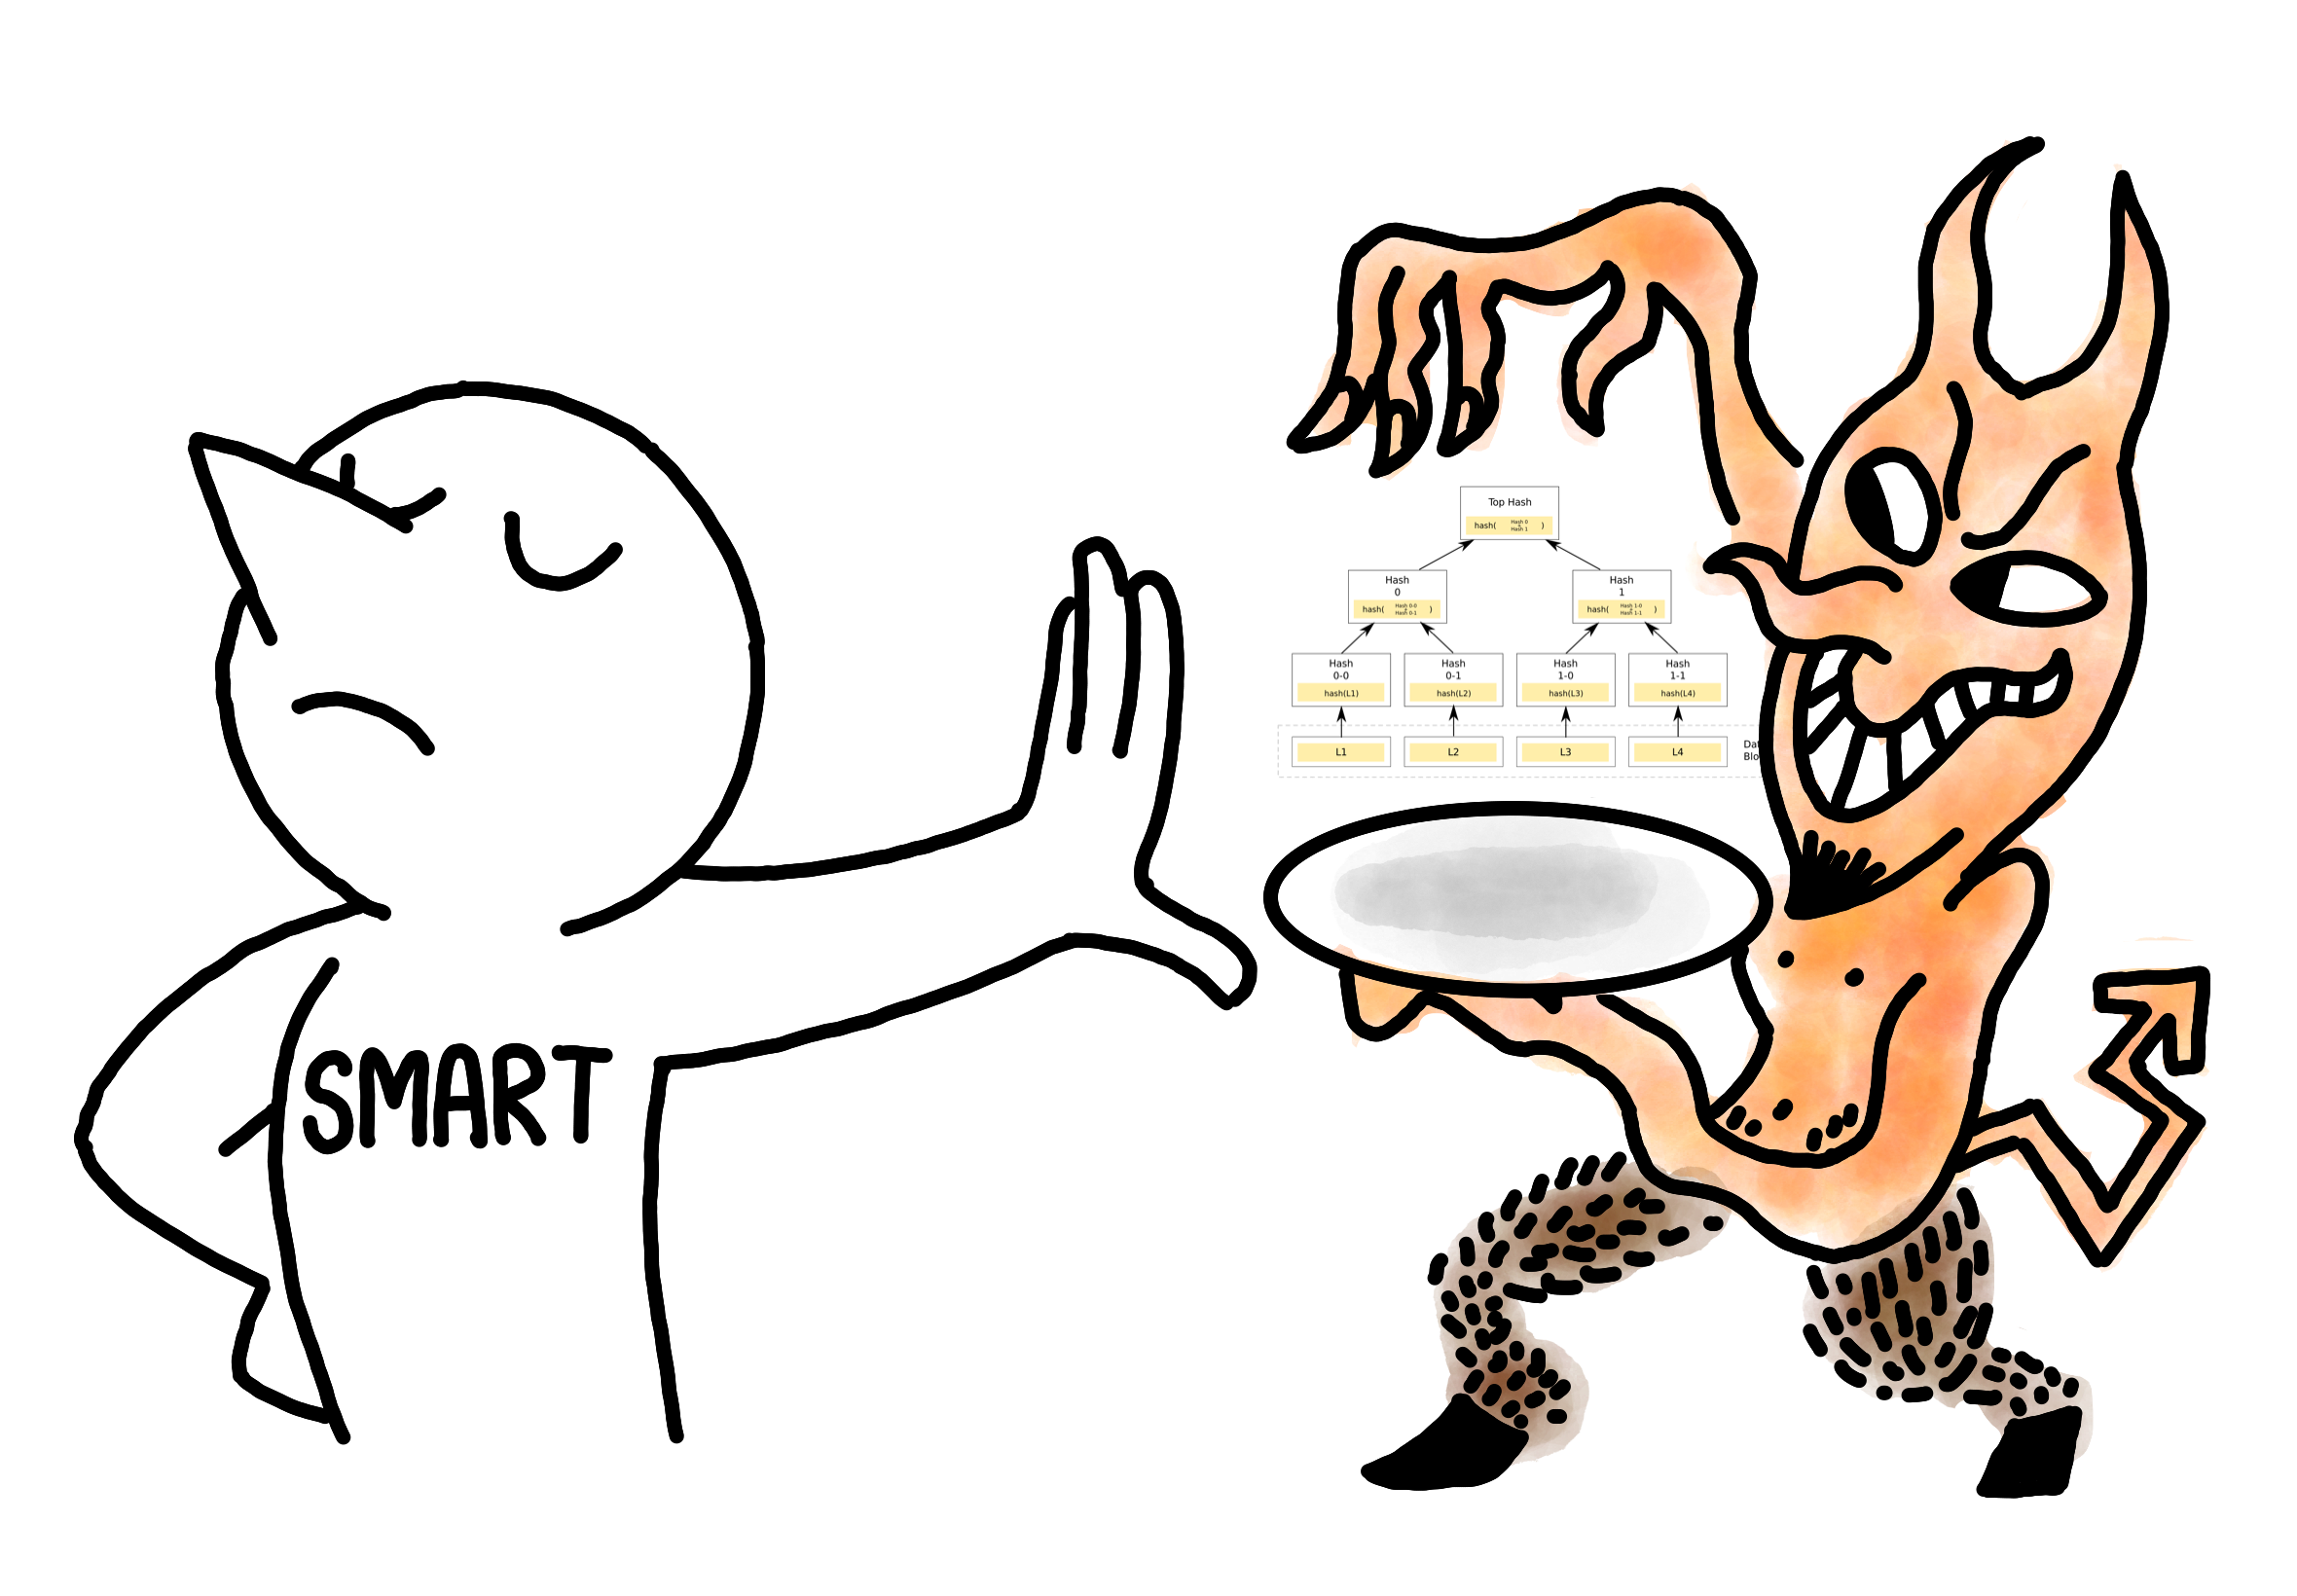
\includegraphics[keepaspectratio=true,width=11.0cm]{sayNoToMerkleTrees.png}
    Drawing: Sam Gwilym 
\end{frame}

\begin{frame}{Order-Statistic Trees\only<2->{ $[\examplec, \examplei)$}}
    \begin{tikzpicture}[xscale=0.95,yscale=1.6][font=\footnotesize]
        \pgfdeclarelayer{background}
        \pgfdeclarelayer{foreground}
        \pgfsetlayers{background,main,foreground}

        \begin{pgfonlayer}{main}
            \node (v00) at (0, 0) [treenodeSmall] {\labeledvalue{$1$}{\examplea}};
            \node (v10) at (1, 0) [treenodeSmall] {\labeledvalue{$1$}{\exampleb}};
            \node (v20) at (2, 0) [treenodeSmall] {\labeledvalue{$1$}{\examplec}};
            \node (v30) at (3, 0) [treenodeSmall] {\labeledvalue{$1$}{\exampled}};
            \node (v40) at (4, 0) [treenodeSmall] {\labeledvalue{$1$}{\examplee}};
            \node (v50) at (5, 0) [treenodeSmall] {\labeledvalue{$1$}{\examplef}};
            \node (v60) at (6, 0) [treenodeSmall] {\labeledvalue{$1$}{\exampleg}};
            \node (v80) at (8, 0) [treenodeSmall] {\labeledvalue{$1$}{\exampleh}};
            % \node (v90) at (9, 0) [treenodeSmall] {\labeledvalue{$1$}{\examplei}};
            \node (v100) at (10, 0) [treenodeSmall] {\labeledvalue{$1$}{\examplei}};
            \node (v110) at (11, 0) [treenodeSmall] {\labeledvalue{$1$}{\examplej}};
        
            \node (v01) at (0.5, 1) [treenode] {$2$};
            \node (v11) at (2.5, 1) [treenode] {$2$};
            \node (v21) at (4.5, 1) [treenode] {$2$};
            \node (v31) at (6, 1) [treenode] {$1$};
            \node (v41) at (8, 1) [treenode] {$1$};
            \node (v51) at (10.5, 1) [treenode] {$2$};
        
            \node (v02) at (1.5, 2) [treenode] {$4$};
            \node (v12) at (5.5, 2) [treenode] {$3$};
            \node (v22) at (9.5, 2) [treenode] {$3$};
        
            \node (v03) at (3.5, 3) [treenode] {$7$};
            \node (v13) at (9.5, 3) [treenode] {$7$};

            \node (v04) at (7.5, 4) [treenode] {$14$};
        
            \draw (v00) edge[edge] (v01);
            \draw (v10) edge[edge] (v01);
            \draw (v20) edge[edge] (v11);
            \draw (v30) edge[edge] (v11);
            \draw (v40) edge[edge] (v21);
            \draw (v50) edge[edge] (v21);
            \draw (v60) edge[edge] (v31);
            \draw (v80) edge[edge] (v41);
            \draw (v100) edge[edge] (v51);
            \draw (v110) edge[edge] (v51);
        
            \draw (v01) edge[edge] (v02);
            \draw (v11) edge[edge] (v02);
            \draw (v21) edge[edge] (v12);
            \draw (v31) edge[edge] (v12);
            \draw (v41) edge[edge] (v22);
            \draw (v51) edge[edge] (v22);
            
            \draw (v02) edge[edge] (v03);
            \draw (v12) edge[edge] (v03);
            \draw (v22) edge[edge] (v13);

            \draw (v03) edge[edge] (v04);
            \draw (v13) edge[edge] (v04);
        \end{pgfonlayer}

        \begin{pgfonlayer}{foreground}
            \only<2->{
                \draw[draw=black, fill=black, opacity=0.6] (-0.5,-0.5) rectangle (1.5,4.5);
                \draw[draw=black, fill=black, opacity=0.6] (9.5,-0.5) rectangle (11.5,4.5);
            }
        \end{pgfonlayer}

        \begin{pgfonlayer}{background}
            \begin{scope}[transparency group, opacity=0.4]
                \only<4->{
                    \draw[draw=orange, fill=orange] (7.1,3.75) rectangle ++(0.8,0.5);
                }

                \only<5->{
                    \draw[orange,line width=11pt,rounded corners=0.1em,line cap=round] (v04.center) -- (v03.center) -- (v02.center) -- (v11.center) -- (v20.center);
                    \draw[orange,line width=11pt,rounded corners=1em,line cap=round] (v04.center) -- (v03.center) -- (v02.center) -- (v11.center) -- (v20.center);

                    \draw[orange,line width=11pt,rounded corners=0.1em,line cap=round] (v04.center) -- (v13.center) -- (v22.center) -- (v51.center) -- (v100.center);
                    \draw[orange,line width=11pt,rounded corners=1em,line cap=round] (v04.center) -- (v13.center) -- (v22.center) -- (v51.center) -- (v100.center);
                }                

                \only<3->{
                    \draw[draw=violet, fill=violet] (2.1,0.75) rectangle ++(0.8,0.5);
                    \draw[draw=violet, fill=violet] (5.1,1.75) rectangle ++(0.8,0.5);
                    \draw[draw=violet, fill=violet] (7.6,0.75) rectangle ++(0.8,0.5);
                }
            \end{scope}
        \end{pgfonlayer}
    \end{tikzpicture}
\end{frame}

\begin{frame}{Monoid Trees}
    \only<2->{Monoid:}
    \begin{itemize}
        \item set of labels: $\N$
        \item binary associative function: $+$
        \item neutral element: $0$\pause\pause
        \item lifting into the monoid: $\lambda x.1$
    \end{itemize}
    \vfill
    \begin{itemize}
        \item<4-> set of labels: $\set{n \st 0 <= n < 2^{256} - 1}$
        \item<5-> binary associative function: xor
        \item<5-> neutral element: $0$
        \item<4-> lifting into the monoid: sha256
    \end{itemize}
\end{frame}

\begin{frame}{Resulting Functions}
    Let $U$ be a set, $\preceq$ a linear order on $U$, $\mathcal{M} = (M, \groupaddsym, \neutraladd)$ a monoid, and $\fun{\h}{U}{M}$.

    We \defined{lift $\h$ to finite sets via $\mathcal{M}$} to obtain $\partialfun{\lift{\h}{\mathcal{M}}}{\powerset{U}}{M}$ with:

    \begin{align*}
    \lift{\h}{\mathcal{M}}(\emptyset) &\defeq \neutraladd,\\
    \lift{\h}{\mathcal{M}}(S) &\defeq \h\bigl(\min(S)\bigr) \oplus \lift{\h}{\mathcal{M}}\bigl(S \setminus \set{\min(S)}\bigr).\\
    \end{align*}

    That is: $\lift{\h}{\mathcal{M}}(S) = \groupadd{\h(s_1)}{\groupadd{\h(s_2)}{\groupadd{\cdots}{\h(s_{\abs{S}})}}}$.
\end{frame}

\begin{frame}{Advantages}
    \begin{itemize}
        \item solid worst-case communication complexity
        \item implementation independence
    \end{itemize}
\end{frame}

\begin{frame}{Alternative Datastructures}
    \begin{tikzpicture}[xscale=1.5,yscale=1.6][font=\footnotesize]
        \pgfdeclarelayer{background}
        \pgfdeclarelayer{foreground}
        \pgfsetlayers{background,main,foreground}

        \begin{pgfonlayer}{main}
            \node (v00) at (0, 0) [treenodeSmall] {\labeledvalue{$1$}{\examplea}};
            \node (v10) at (1, 0) [treenodeSmall] {\labeledvalue{$1$}{\examplec}};
            \node (v20) at (2, 0) [treenodeSmall] {\labeledvalue{$1$}{\examplee}};
            \node (v30) at (3, 0) [treenodeSmall] {\labeledvalue{$1$}{\exampleg}};
            \node (v40) at (4, 0) [treenodeSmall] {\labeledvalue{$1$}{\examplei}};
            \node (v50) at (5, 0) [treenodeSmall] {\labeledvalue{$1$}{\examplek}};
            \node (v60) at (6, 0) [treenodeSmall] {\labeledvalue{$1$}{\examplem}};
        
            \node (v01) at (0.5, 1) [treenodeSmall] {\labeledvalue{$3$}{\exampleb}};
            \node (v11) at (2.5, 1) [treenodeSmall] {\labeledvalue{$3$}{\examplef}};
            \node (v21) at (4.5, 1) [treenodeSmall] {\labeledvalue{$3$}{\examplej}};
            \node (v31) at (6.5, 1) [treenodeSmall] {\labeledvalue{$2$}{\examplen}};
        
            \node (v02) at (1.5, 2) [treenodeSmall] {\labeledvalue{$7$}{\exampled}};
            \node (v12) at (5.5, 2) [treenodeSmall] {\labeledvalue{$6$}{\examplel}};
        
            \node (v03) at (3.5, 3) [treenode] {\labeledvalue{$14$}{\exampleh}};
        
            \draw (v00) edge[edge] (v01);
            \draw (v10) edge[edge] (v01);
            \draw (v20) edge[edge] (v11);
            \draw (v30) edge[edge] (v11);
            \draw (v40) edge[edge] (v21);
            \draw (v50) edge[edge] (v21);
            \draw (v60) edge[edge] (v31);
        
            \draw (v01) edge[edge] (v02);
            \draw (v11) edge[edge] (v02);
            \draw (v21) edge[edge] (v12);
            \draw (v31) edge[edge] (v12);
            
            \draw (v02) edge[edge] (v03);
            \draw (v12) edge[edge] (v03);
        \end{pgfonlayer}

        \begin{pgfonlayer}{foreground}
            \only<2->{
                \draw[draw=black, fill=black, opacity=0.6] (-0.5,-0.5) rectangle (0.8,4.5);
                \draw[draw=black, fill=black, opacity=0.6] (4.8,-0.5) rectangle (8.5,4.5);
            }
        % \end{pgfonlayer}

        % \begin{pgfonlayer}{background}
            \begin{scope}[transparency group, opacity=0.3]
                \only<5->{
                    \draw[orange,line width=11pt,rounded corners=0.1em,line cap=round] (v03.center) -- (v02.center) -- (v01.center) -- (v10.center);
                    \draw[orange,line width=11pt,rounded corners=1em,line cap=round] (v03.center) -- (v02.center) -- (v01.center) -- (v10.center);
                    \draw[orange,line width=11pt,rounded corners=0.1em,line cap=round] (v03.center) -- (v12.center) -- (v21.center) -- (v50.center);
                    \draw[orange,line width=11pt,rounded corners=1em,line cap=round] (v03.center) -- (v12.center) -- (v21.center) -- (v50.center);
                }                

                \only<3->{
                    \draw[draw=violet, fill=violet] (0.7,-0.05) rectangle ++(0.6,0.5);
                    \draw[draw=violet, fill=violet] (2.2,0.95) rectangle ++(0.6,0.5);
                    \draw[draw=violet, fill=violet] (3.7,-0.05) rectangle ++(0.6,0.5);
                }

                \only<4->{
                    \draw[draw=blue, fill=blue] (1.2,1.6) rectangle ++(0.6,0.42);
                    \draw[draw=blue, fill=blue] (3.1,2.63) rectangle ++(0.8,0.42);
                    \draw[draw=blue, fill=blue] (4.2,0.6) rectangle ++(0.6,0.42);
                }
            \end{scope}
        \end{pgfonlayer}
    \end{tikzpicture}
\end{frame}

\begin{frame}{Alternative Datastructures}
    \begin{itemize}
        \item monoid B-Tree
        \item monoid prefix tree
        \item monoid skip list
        \item monoid zip-tree
        \item no datastructure at all
        \item ...
    \end{itemize}
\end{frame}

\begin{frame}{Successive Ranges}
    \begin{tikzpicture}[xscale=1.4,yscale=1.6][font=\footnotesize]
        \pgfdeclarelayer{background}
        \pgfdeclarelayer{foreground}
        \pgfsetlayers{background,main,foreground}

        \begin{pgfonlayer}{background}
            \node (v00) at (0, 0) [treenodeSmall] {\labeledvalue{$1$}{\examplea}};
            \node (v10) at (1, 0) [treenodeSmall] {\labeledvalue{$1$}{\exampleb}};
            \node (v20) at (2, 0) [treenodeSmall] {\labeledvalue{$1$}{\examplec}};
            \node (v30) at (3, 0) [treenodeSmall] {\labeledvalue{$1$}{\exampled}};
            \node (v40) at (4, 0) [treenodeSmall] {\labeledvalue{$1$}{\examplee}};
            \node (v50) at (5, 0) [treenodeSmall] {\labeledvalue{$1$}{\examplef}};
            \node (v60) at (6, 0) [treenodeSmall] {\labeledvalue{$1$}{\exampleg}};
            \node (v70) at (7, 0) [treenodeSmall] {\labeledvalue{$1$}{\exampleh}};
        
            \node (v01) at (0.5, 1) [treenode] {$2$};
            \node (v11) at (2.5, 1) [treenode] {$2$};
            \node (v21) at (4.5, 1) [treenode] {$2$};
            \node (v31) at (6.5, 1) [treenode] {$2$};
        
            \node (v02) at (1.5, 2) [treenode] {$4$};
            \node (v12) at (5.5, 2) [treenode] {$4$};
        
            \node (v03) at (3.5, 3) [treenode] {$8$};
        
            \draw (v00) edge[edge] (v01);
            \draw (v10) edge[edge] (v01);
            \draw (v20) edge[edge] (v11);
            \draw (v30) edge[edge] (v11);
            \draw (v40) edge[edge] (v21);
            \draw (v50) edge[edge] (v21);
            \draw (v60) edge[edge] (v31);
            \draw (v70) edge[edge] (v31);
        
            \draw (v01) edge[edge] (v02);
            \draw (v11) edge[edge] (v02);
            \draw (v21) edge[edge] (v12);
            \draw (v31) edge[edge] (v12);
            
            \draw (v02) edge[edge] (v03);
            \draw (v12) edge[edge] (v03);
        \end{pgfonlayer}

        \begin{pgfonlayer}{main}
            \draw[draw=black, fill=black, opacity=0.6] (-0.5,-0.5) rectangle ++(1,4);
            \draw[draw=blue, fill=blue, opacity=0.1] (0.5,-0.5) rectangle ++(2,4);
            \draw[draw=red, fill=red, opacity=0.1] (2.5,-0.5) rectangle ++(2,4);
            \draw[draw=yellow, fill=yellow, opacity=0.1] (4.5,-0.5) rectangle ++(2,4);
            \draw[draw=black, fill=black, opacity=0.6] (6.5,-0.5) rectangle ++(1,4);
        \end{pgfonlayer}

        \begin{pgfonlayer}{foreground}
            \only<2-3>{
                \draw [-latex,color=blue,ultra thick] ($(v03.center)!0.15!(v02.center)$) -- ($(v03.center)!0.85!(v02.center)$);
                \draw [-latex,color=blue,ultra thick] ($(v02.center)!0.15!(v01.center)$) -- ($(v02.center)!0.75!(v01.center)$);
                \draw [-latex,color=blue,ultra thick] ($(v01.center)!0.15!(v10.center)$) -- ($(v01.center)!0.55!(v10.center)$);
                \draw [-latex,color=blue,ultra thick] ($(v03.center)!0.15!(v02.center)+(-0.15,0.15)$) -- ($(v03.center)!0.85!(v02.center)+(-0.15,0.15)$);
                \draw [-latex,color=blue,ultra thick] ($(v02.center)!0.15!(v11.center)$) -- ($(v02.center)!0.75!(v11.center)$);
                \draw [-latex,color=blue,ultra thick] ($(v11.center)!0.15!(v20.center)$) -- ($(v11.center)!0.55!(v20.center)$);
            }
            \only<3>{
                \draw [-latex,color=red,ultra thick] ($(v03.center)!0.15!(v02.center)+(0.15,-0.15)$) -- ($(v03.center)!0.85!(v02.center)+(0.15,-0.15)$);
                \draw [-latex,color=red,ultra thick] ($(v02.center)!0.15!(v11.center)+(0.15,0.15)$) -- ($(v02.center)!0.75!(v11.center)+(0.15,0.15)$);
                \draw [-latex,color=red,ultra thick] ($(v11.center)!0.15!(v30.center)$) -- ($(v11.center)!0.55!(v30.center)$);
            }
            \only<3>{
                \draw [-latex,color=red,ultra thick] ($(v03.center)!0.15!(v12.center)+(-0.15,-0.15)$) -- ($(v03.center)!0.85!(v12.center)+(-0.15,-0.15)$);
                \draw [-latex,color=red,ultra thick] ($(v12.center)!0.15!(v21.center)+(-0.15,0.15)$) -- ($(v12.center)!0.75!(v21.center)+(-0.15,0.15)$);
                \draw [-latex,color=red,ultra thick] ($(v21.center)!0.15!(v40.center)$) -- ($(v21.center)!0.55!(v40.center)$);

                \draw [-latex,color=brown,ultra thick] ($(v03.center)!0.15!(v12.center)$) -- ($(v03.center)!0.85!(v12.center)$);
                \draw [-latex,color=brown,ultra thick] ($(v12.center)!0.15!(v21.center)$) -- ($(v12.center)!0.75!(v21.center)$);
                \draw [-latex,color=brown,ultra thick] ($(v21.center)!0.15!(v50.center)$) -- ($(v21.center)!0.55!(v50.center)$);

                \draw [-latex,color=brown,ultra thick] ($(v03.center)!0.15!(v12.center)+(0.15,0.15)$) -- ($(v03.center)!0.85!(v12.center)+(0.15,0.15)$);
                \draw [-latex,color=brown,ultra thick] ($(v12.center)!0.15!(v31.center)$) -- ($(v12.center)!0.75!(v31.center)$);
                \draw [-latex,color=brown,ultra thick] ($(v31.center)!0.15!(v60.center)$) -- ($(v31.center)!0.55!(v60.center)$);
            }

            \only<4->{
                \draw [-latex,color=blue,ultra thick] ($(v01.center)!0.55!(v10.center)+(0.1,0)$) -- ($(v01.center)!0.15!(v10.center)+(0.1,0)$);
                \draw [-latex,color=blue,ultra thick] ($(v02.center)!0.75!(v01.center)+(0.1,0)$) -- ($(v02.center)!0.15!(v01.center)+(0.1,0)$);
                \draw [-latex,color=blue,ultra thick] ($(v02.center)!0.15!(v11.center)+(-0.1,0)$) -- ($(v02.center)!0.75!(v11.center)+(-0.1,0)$);
                \draw [-latex,color=blue,ultra thick] ($(v11.center)!0.2!(v20.center)+(-0.1,0)$) -- ($(v11.center)!0.55!(v20.center)+(-0.1,0)$);
            }
            \only<5->{
                \draw [-latex,color=red,ultra thick] ($(v11.center)!0.55!(v20.center)+(0.1,0)$) -- ($(v11.center)!0.2!(v20.center)+(0.1,0)$);
                \draw [-latex,color=red,ultra thick] ($(v11.center)!0.2!(v30.center)+(-0.1,0)$) -- ($(v11.center)!0.55!(v30.center)+(-0.1,0)$);
            }
            \only<5->{
                \draw [-latex,color=red,ultra thick] ($(v11.center)!0.55!(v30.center)+(0.1,0)$) -- ($(v11.center)!0.2!(v30.center)+(0.1,0)$);
                \draw [-latex,color=red,ultra thick] ($(v02.center)!0.75!(v11.center)+(0.1,0)$) -- ($(v02.center)!0.15!(v11.center)+(0.1,0)$);
                \draw [-latex,color=red,ultra thick] ($(v03.center)!0.85!(v02.center)+(0.1,0)$) -- ($(v03.center)!0.15!(v02.center)+(0.1,0)$);

                \draw [-latex,color=red,ultra thick] ($(v03.center)!0.15!(v12.center)+(-0.1,0)$) -- ($(v03.center)!0.85!(v12.center)+(-0.1,0)$);
                \draw [-latex,color=red,ultra thick] ($(v12.center)!0.15!(v21.center)+(-0.1,0)$) -- ($(v12.center)!0.75!(v21.center)+(-0.1,0)$);
                \draw [-latex,color=red,ultra thick] ($(v21.center)!0.2!(v40.center)+(-0.1,0)$) -- ($(v21.center)!0.55!(v40.center)+(-0.1,0)$);
            }

            \only<5->{
                \draw [-latex,color=brown,ultra thick] ($(v21.center)!0.55!(v40.center)+(0.1,0)$) -- ($(v21.center)!0.2!(v40.center)+(0.1,0)$);
                \draw [-latex,color=brown,ultra thick] ($(v21.center)!0.2!(v50.center)+(-0.1,0)$) -- ($(v21.center)!0.55!(v50.center)+(-0.1,0)$);

                \draw [-latex,color=brown,ultra thick] ($(v21.center)!0.55!(v50.center)+(0.1,0)$) -- ($(v21.center)!0.2!(v50.center)+(0.1,0)$);
                \draw [-latex,color=brown,ultra thick] ($(v12.center)!0.75!(v21.center)+(0.1,0)$) -- ($(v12.center)!0.15!(v21.center)+(0.1,0)$);

                \draw [-latex,color=brown,ultra thick] ($(v12.center)!0.15!(v31.center)+(-0.1,0)$) -- ($(v12.center)!0.75!(v31.center)+(-0.1,0)$);
                \draw [-latex,color=brown,ultra thick] ($(v31.center)!0.2!(v60.center)+(-0.1,0)$) -- ($(v31.center)!0.55!(v60.center)+(-0.1,0)$);
            }
        \end{pgfonlayer}
    \end{tikzpicture}
\end{frame}

\begin{frame}{Some Peers Are Out To Get Us}
    \begin{itemize}
        \item adversary must sabotage reconciliation
        \item<2-> active and passive adversaries
        \item<3-> randomized boundaries defeat individual collisions 
        \item<4-> better protection: secure hash functions
    \end{itemize}
\end{frame}

\begin{frame}{Secure Hash Functions}
    Let $U$ be a set, $\mathcal{M} = (M, \groupaddsym, \neutraladd)$ a monoid, and $\fun{\f}{\powerset{U}}{M}$.

    $\f$ is \defined{set-homomorphic} if $\f(U_1 \cup U_2) = \f(U_1) \groupaddsym \f(U_2)$.\pause

    \sout{xor}, \sout{addition}, multiplication, lattices, RSA, eliptic curves.\pause

    Our functions: $\lift{\h}{\mathcal{M}}(S) = \groupadd{\h(s_1)}{\groupadd{\h(s_2)}{\groupadd{\cdots}{\h(s_{\abs{S}})}}}$\pause

    \vfill

    Let further $\preceq$ a linear order on $U$.
	
	$\h$ is a \defined{\somewhatmorphism{}} if for $S_0, S_1 \in \powerset{U}$ with $\max(S_0) \prec \min(S_1)$, we have $\h(S_0 \cup S_1) = \groupadd{\h(S_0)}{\h(S_1)}$.

    \vfill

    \pause{}No commutativity: Cayley hash functions
\end{frame}

\begin{frame}{Summary}
    \begin{itemize}
        \item divide-and-conquer to find differences by checking fingerprint equality
        \item tree-friendly functions allow for efficient and flexible implementation
        \item cryptographically secure tree-friendly functions exist
        \item pretty simple compared to traditional solutions\pause
        \item remember to say no to Merkle trees
    \end{itemize}
\end{frame}

\begin{frame}{Bonus Slides!}
    
\end{frame}

\begin{frame}{Reducing Computation Times}
    \begin{itemize}
        \item Step 1: Put a Merkle tree on it
        \item Step 2: ???
        \item Step 3: Profit
    \end{itemize}

    \vfill

    Auvolat, Alex, and François Taïani. "Merkle search trees: Efficient state-based CRDTs in open networks." 2019 38th Symposium on Reliable Distributed Systems (SRDS). IEEE, 2019.
\end{frame}

\begin{frame}{Merkle Trees}
    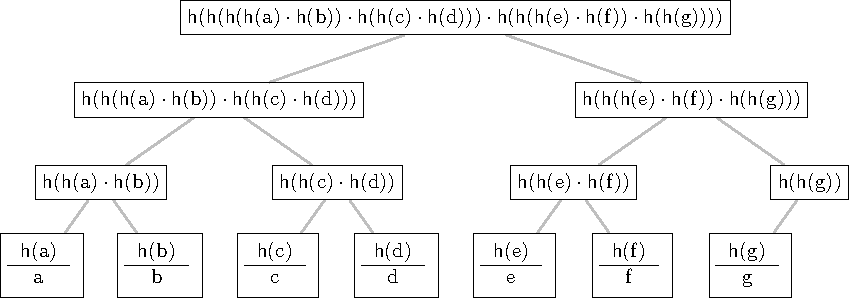
\includegraphics[keepaspectratio=true,width=11.4cm]{merkle1.pdf}
\end{frame}

\begin{frame}{Merkle Trees}
    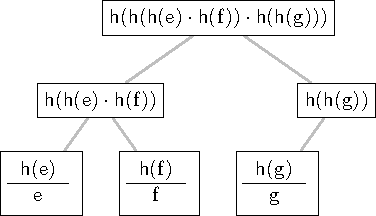
\includegraphics[keepaspectratio=true,width=5cm]{merkle2.pdf}\hfill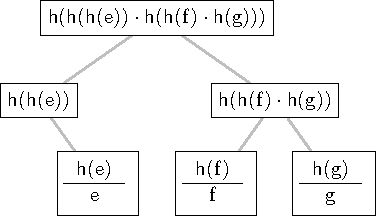
\includegraphics[keepaspectratio=true,width=5cm]{merkle3.pdf}
\end{frame}

\begin{frame}{Merkle Tree Reconciliation}
    \begin{tikzpicture}[xscale=1.6,yscale=0.95][font=\footnotesize]
        \alt<1->{\node (v00) at (0, 0) [treenodeEqual] {\labeledvalue{$147$}{\examplea}};}{\node (v00) at (0, 0) [treenode] {\labeledvalue{$147$}{\examplea}};};
        \alt<1->{\node (v10) at (1, 0) [treenodeUnequal] {\labeledvalue{$821$}{\exampleb}};}{\node (v10) at (1, 0) [treenode] {\labeledvalue{$821$}{\exampleb}};};
        \alt<1->{\node (v30) at (3, 0) [treenodeEqual] {\labeledvalue{$165$}{\exampled}};}{\node (v30) at (3, 0) [treenode] {\labeledvalue{$165$}{\exampled}};};
        \node (v40) at (4, 0) [treenode] {\labeledvalue{$508$}{\examplee}};
        \node (v50) at (5, 0) [treenode] {\labeledvalue{$681$}{\examplef}};
        \node (v60) at (6, 0) [treenode] {\labeledvalue{$570$}{\exampleg}};
    
        \alt<1->{\node (v01) at (0.5, 1) [treenodeUnequal] {$299$};}{\node (v01) at (0.5, 1) [treenode] {$299$};};
        \alt<1->{\node (v11) at (2.5, 1) [treenodeUnequal] {$212$};}{\node (v11) at (2.5, 1) [treenode] {$212$};};
        \node (v21) at (4.5, 1) [treenode] {$996$};
        \node (v31) at (6.5, 1) [treenode] {$974$};
    
        \alt<1->{\node (v02) at (1.5, 2) [treenodeUnequal] {$772$};}{\node (v02) at (1.5, 2) [treenode] {$772$};};
        \alt<1->{\node (v12) at (5.5, 2) [treenodeEqual] {$336$};}{\node (v12) at (5.5, 2) [treenode] {$336$};};
    
        \alt<1->{\node (v03) at (3.5, 3) [treenodeUnequal] {$242$};}{\node (v03) at (3.5, 3) [treenode] {$242$};};
    
        \draw (v00) edge[edge] (v01);
        \draw (v10) edge[edge] (v01);
        \draw (v30) edge[edge] (v11);
        \draw (v40) edge[edge] (v21);
        \draw (v50) edge[edge] (v21);
        \draw (v60) edge[edge] (v31);
    
        \draw (v01) edge[edge] (v02);
        \draw (v11) edge[edge] (v02);
        \draw (v21) edge[edge] (v12);
        \draw (v31) edge[edge] (v12);
        
        \draw (v02) edge[edge] (v03);
        \draw (v12) edge[edge] (v03);
    \end{tikzpicture}

    \begin{tikzpicture}[xscale=1.6,yscale=0.95][font=\footnotesize]
        \alt<1->{\node (v00) at (0, 0) [treenodeEqual] {\labeledvalue{$147$}{\examplea}};}{\node (v00) at (0, 0) [treenode] {\labeledvalue{$147$}{\examplea}};};
        \alt<1->{\node (v20) at (2, 0) [treenodeUnequal] {\labeledvalue{$260$}{\examplec}};}{\node (v20) at (2, 0) [treenode] {\labeledvalue{$260$}{\examplec}};};
        \alt<1->{\node (v30) at (3, 0) [treenodeEqual] {\labeledvalue{$165$}{\exampled}};}{\node (v30) at (3, 0) [treenode] {\labeledvalue{$165$}{\exampled}};};
        \node (v40) at (4, 0) [treenode] {\labeledvalue{$508$}{\examplee}};
        \node (v50) at (5, 0) [treenode] {\labeledvalue{$681$}{\examplef}};
        \node (v60) at (6, 0) [treenode] {\labeledvalue{$570$}{\exampleg}};
    
        \alt<1->{\node (v01) at (0.5, 1) [treenodeUnequal] {$089$};}{\node (v01) at (0.5, 1) [treenode] {$089$};};
        \alt<1->{\node (v11) at (2.5, 1) [treenodeUnequal] {$602$};}{\node (v11) at (2.5, 1) [treenode] {$602$};};
        \node (v21) at (4.5, 1) [treenode] {$996$};
        \node (v31) at (6.5, 1) [treenode] {$974$};
    
        \alt<1->{\node (v02) at (1.5, 2) [treenodeUnequal] {$446$};}{\node (v02) at (1.5, 2) [treenode] {$446$};};
        \alt<1->{\node (v12) at (5.5, 2) [treenodeEqual] {$336$};}{\node (v12) at (5.5, 2) [treenode] {$336$};};
    
        \alt<1->{\node (v03) at (3.5, 3) [treenodeUnequal] {$571$};}{\node (v03) at (3.5, 3) [treenode] {$571$};};
    
        \draw (v00) edge[edge] (v01);
        \draw (v20) edge[edge] (v11);
        \draw (v30) edge[edge] (v11);
        \draw (v40) edge[edge] (v21);
        \draw (v50) edge[edge] (v21);
        \draw (v60) edge[edge] (v31);
    
        \draw (v01) edge[edge] (v02);
        \draw (v11) edge[edge] (v02);
        \draw (v21) edge[edge] (v12);
        \draw (v31) edge[edge] (v12);
        
        \draw (v02) edge[edge] (v03);
        \draw (v12) edge[edge] (v03);
    \end{tikzpicture}
\end{frame}

\begin{frame}{Merkle Tree Reconciliation}
    \begin{itemize}
        \item inflexible data representation
        \item inacceptable worst-case complexity \begin{itemize}
            \item remember, some peers are out to get us
        \end{itemize}
    \end{itemize}
\end{frame}

\end{document}
